\setAuthor{}
\setRound{lõppvoor}
\setYear{2019}
\setNumber{G 10}
\setDifficulty{10}
\setTopic{TODO}

\prob{Pöörduv elektriväli}
Elektriväli $\vec E$ muudab perioodiga $4T$ oma suunda pöördudes $x-y$-tasandis iga 
ajavahemiku $T$ möödudes hüppeliselt $\SI{90}\degree$ päripäeva. Seega, kui $t$ tähistab aega 
ning $\hat x$ ja $\hat y$ tähistavad vastavalt $x$- ja $y$-telje sihilisi ühikvektoreid,  siis ajavahemikel
\begin{align*}
4nT\le &t < 4nT+T \;\; & \vec E&=E_0\hat x,\\
4nT+T\le &t < 4nT+2T   & \vec E&=-E_0\hat y,\\
4nT+2T\le &t < 4nT+3T  & \vec E&=-E_0\hat x \;\;\mbox{ja}\\
4nT+3T\le &t < 4nT+4T & \vec E&=E_0\hat y.
\end{align*}

On teada, et osake massiga $m$ ja laenguga $q$ liigub perioodiliselt, st mööda kinnist trajektoori; visandage selle osakese 
trajektoor $x-y$-tasandis ja leidke trajetoori $x$-telje sihiline läbimõõt. 

\hint

\solu
Et osakese $x$-telje sihiline keskmine kiirus $v_x$ oleks null, peab ajaperioodidel $4nT+T\le t < 4nT+2T$ ja  $4nT+3T\le t < 4nT+4T$ olema $v_x$ väärtused võrdsed ja vastasmärgilised, vastavalt $u$ ja $-u$; ajavahemikul $4nT+2T\le t < 4nT+3T$ annab elektriväli osakesele $x$-suunalise impulsi $-E_0qT$, seetõttu
$$2mu=E_0qT \;\;\Rightarrow\;\; u=\frac{E_0qT}{2m}.$$
Järgneva veerandperioodi jooksul püsib osakese $x$-sihiline kiirus konstantselt võrdne $u$-ga ning seega nihkub osake sel ajal $x$-telje sihis $x_1=uT$ võrra. Järgneva kaheksandikperioodi jooksul (ketusega $T/2$) kahaneb kiirus lineaarselt ajas nullini, seetõttu on täiendav nihe leitav keskmise kiiruse $\frac u2$ abil, $x_2=\frac u2\cdot \frac T2=uT/4$; sümmeetria tõttu toimus samasugune nihe ka konstantse kiirusega veerandperioodile eelenenud kaheksandikperioodi jooksul, st kogunihe (ja seega trajektoori $x$-telje sihiline läbimõõt) on $$x_1+2x_2=\frac32 uT=\frac{3E_0qT^2}{4m}.$$
Sümmeetria tõttu on $y$-telje sihiline läbimõõt samasugune. Trajektooriks on kujund, mis koosneb neljast paraboolist --- iga järgmine parabool on saadud eelmisest täisnurga võrra pööramisel (paraboolide pikkused peavad olema sellised, et otspunktides oleks tõusnurk $45^\circ$: kõverad peavad liituma ilma murdepunktita.

\vspace{-20pt}
\begin{center}
  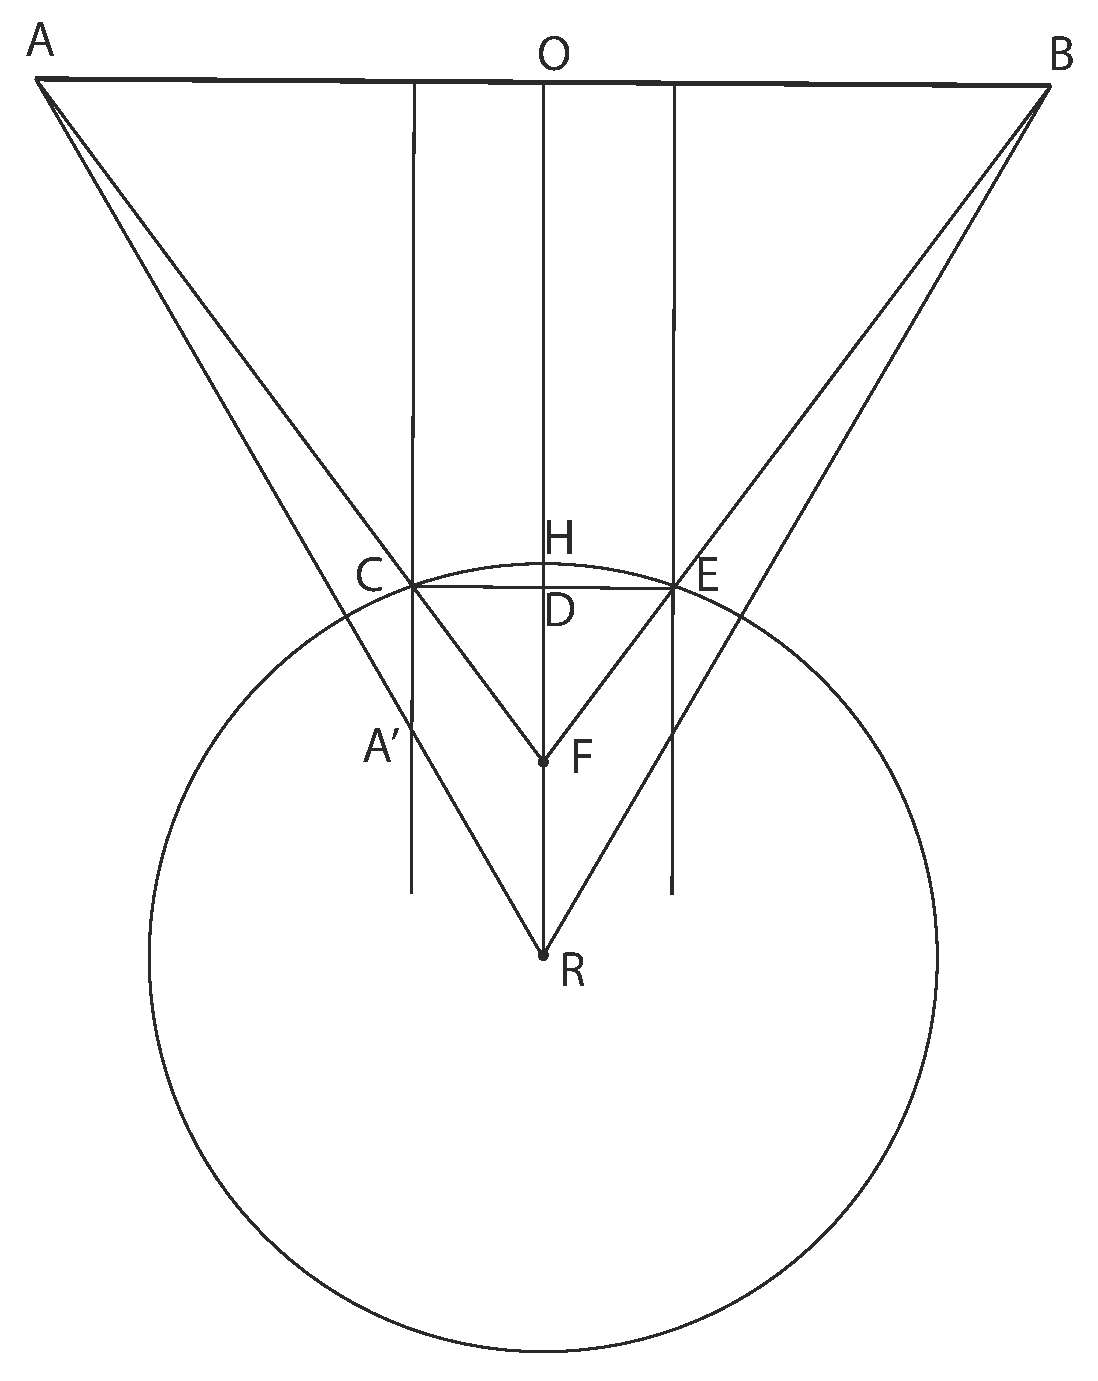
\includegraphics[width=0.6\textwidth]{2019-v3g-10-yl.pdf}
\end{center}
\vspace{-20pt}
\probend